\documentclass[11pt]{article}
\usepackage[nomarkers,figuresonly]{endfloat}
\usepackage{tkz-graph}
\usetikzlibrary{shapes.geometric}

\title{Optimal Dub-E Scheduling}
\author{Skyler Peterson, Alex Sanchez-Stern}

\begin{document}
\maketitle
\section{Introduction}
For our final project,
we decided to look to robotics
for problems that SMT might be able to tackle.
Since we are fortunate enough to be at a school
where there is always interesting work going on across fields,
we didn't have to look far.
We contacted Michael Jae-Yoon Chung and Andrzej Pronobis,
who are working on the Semantics Aware Robotic Assistant,
more commonly known as DUB-E.
DUB-E is able to traverse the CSE building,
and accomplish tasks for its users,
such as checking whether a particular professor is in their office.
DUB-E is controlled via a web interface,
from which users can request that certain tasks be accomplished,
by a particular deadline.

Unfortunately, when deadlines are short
and there are many tasks to accomplish,
it is non-trivial to decide what task
should be accomplished and when.
Additionally, the expressive power of the interface to DUB-E
is currently limited;
Users can specify a task deadline,
but cannot specify more precise timing information,
such as a time in the future
before which the task should not be done
or multiple time periods in which a task can be accomplished.
The current implementation is a simple FIFO ordering based on
time of scheduling. No other temporal information is
used. When a task is completed the next is begun and if the
deadline has passed, an apology is sent and the next task
is run.

Handling these new scheduling concerns
requires a more sophisticated scheduling algorithm
than the one that was previously implemented in DUB-E.
We implemented this new scheduling algorithm
by encoding the scheduling constraints into SMT,
and then using Z3 as a backend
to solve the constraints.
The result is a schedule which instructs DUB-E
when to tackle each task and,
when necessary,
how long to wait in between tasks.
This new scheduler allows DUB-E
to take advantage of timing information,
allowing many more tasks to be completed.

\section{Overview}
DUB-E's overall behavior is quite simple.
It is notified of new tasks via the web interface,
and it's scheduler decides what tasks to do when.
Each time it receives a new task,
it can change how it schedules its current tasks.
Tasks which are completed are removed from its schedule.

But not all tasks get completed.
If DUB-E is overscheduled,
it may not have enough time to complete a requested task in time.
Additionally, the travel time of DUB-E
is not entirely predictable.
While its travel time between two locations
can mostly be bounded within a range,
it is always possible that it will completely fail,
and take much longer to reset itself
and become fully operational again.

The previous scheduling algorithm
for DUB-E was quite simple.
DUB-E simply maintained a FIFO queue
upon which it's tasks resided.
New requests made via the web interface
were added to the end of the queue,
and when DUB-E was not currently working on a task,
it pulled the next task from the front of the queue.
When DUB-E does pull a task from the queue
whose deadline had already passed,
it notifies the user that it was unable to complete the task,
and drops it from the queue.
While simple and fair,
this algorithm fails to provide
optimal behavior in a variety of simple scenarios.

Consider the case where user one
requests that DUB-E go the kitchen
and check for food
within the next thirty five minutes.
Let's assume that it takes DUB-E fifteen minutes
to complete this task,
ten minutes to go to the kitchen,
five to check for food.
The, user two requests that DUB-E
check whether Emina Torlak is in her office,
within the next twenty minutes.
It takes again, fifteen minutes total
for DUB-E to complete the task,
ten to arrive at Emina's office,
and five to confirm whether or not she is there.
If DUB-E addresses the tasks in a first come, first serve order,
as the old scheduler would do,
by the time it had finished checking for food,
it would have missed the deadline for finding Emina.
If instead it had reordered the tasks,
checking for Emina first,
it would be able to accomplish both tasks on time.
This scenario can become even worse if user one gives a
very large deadline and a task which takes a long time.
Then if many small tasks are given which all take place in
the same location but also have short deadlines, the first
user has just blocked all of these task unnecessarily.
In the worse case, this can allow a bad user to launch
a DOS, by simply scheduling large tasks.

The DUB-E scheduling problem is not simply
a classic instance of scheduling
where each task takes a fixed amount of time.
Consider the case where DUB-E
is requested to check for both Emina and Zach Tatlock
in their respective offices.
It might be the case that both requests
should be completed in 18 minutes.
If DUB-E is in another part of the building,
it might take five minutes to get to both offices,
and take five minutes to check them.
Taken separately, each request takes ten minutes,
and it is not possible to do both,
since it would take twenty minutes to do both individually.
But Zach's and Emina's offices are only a minute apart,
both being on the fifth floor (see Figure \ref{fig:overview-example}),
it actually is possible to complete both tasks.
DUB-E can go to one office, complete the task,
and travel to the other one,
in only eleven minutes.
Completing the second task takes a further five minutes,
for a total time of sixteen minutes,
well within the deadline.

\begin{figure}
  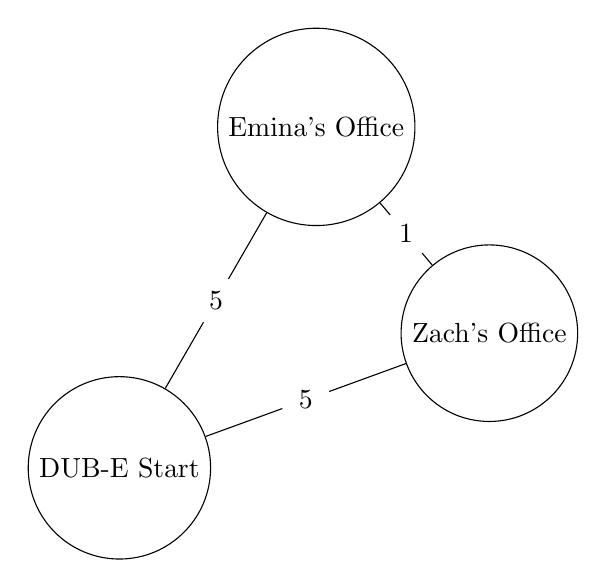
\begin{tikzpicture}
    \tikzstyle{every node}=[draw, shape=circle];
    \node (S) at (0:0) {DUB-E Start};
    \node (Z) at (20:5) {Zach's Office};
    \node (E) at (60:5) {Emina's Office};
    \draw (S) -- (Z) node [midway, fill=white, draw=white] {5};
    \draw (S) -- (E) node [midway, fill=white, draw=white] {5};
    \draw (Z) -- (E) node [midway, fill=white, draw=white] {1};
  \end{tikzpicture}
  \caption{
    Each task takes five minutes
    to get to from the start,
    but they are only one minute apart.
  }
  \label{fig:overview-example}
\end{figure}

It is clear from this example that
a proper scheduling algorithm must consider spatial factors,
as well as temporal ones.
Additionally, it may be the case that not all tasks can be scheduled,
and tasks have non-uniform priorities.
The DUB-E team asked for multiple task priorities,
that were weighted,
so that sufficiently many lower priority tasks
could be chosen over a higher priority task,
but also include a special admin priority
that would never be dropped in favor of lower tasks. An
Admin task may only be dropped if conflicting with another admin
task.


\section{Scheduler Encoding}
To tackle these unique constraints,
we had to develop an encoding which could scale fairly well,
while still supporting all the features the DUB-E team wanted.
Since tasks can occur at a multitude of times,
and include waiting times between tasks
if a task is completed and the next one
belongs to an interval that has not started,
a schedule must contain more than just a list of tasks to be completed;
it also needs to know to wait between certain tasks.

A naive approach would be to ask the solver
to simply give us the times at which each task is done,
given the problem constraints.
But solving for this many continuous variables
would not scale to an even reasonable number of tasks.
Instead, we discretized time into an integer counter,
simplifying the issue even if we lose a little granularity,
and we divided the problem space into assignment of tasks
to ``time steps.''

For finding the optimal schedule of N tasks,
we attempt to find the best assignment
of tasks to N time steps,
as well as solving for a single integer for each time step
indicating how long DUB-E should be waited before starting that time step.
We constrain the solution to this in several ways
which allow results to be a valid schedule.

Since there exists a boolean variable for
each task being accomplished at each step,
we add a one-hot constraint
so that at most one task is scheduled for each step,
and each task is scheduled for at most one step.
It might seem like we should require that
exactly one task be accomplished at each step,
and each task be accomplished at exactly one step.
However, it may be the case that
the tasks are over-constraining,
and so not all of them can be accomplished.
To account for this case,
we must allow for tasks to be not scheduled for any step,
and for some steps to be empty.
We create a boolean variable for each time step t labeled None@t,
which indicates whether or not \textbf{no} tasks are scheduled at that time step,
and require that exactly one of the set of $\{None\} \cup tasksScheduled$
be true for each time step.

To make other constraints simpler,
including the resulting schedule,
we also require that all of the ''None's''
be at the end of the schedule.
That is, if a time step has ‘’None’’,
then all time steps after it have ‘’None’’,
forcing all actual tasks to the front of the time steps.
(see Figure \ref{fig:none-constraints}).
\begin{figure}
  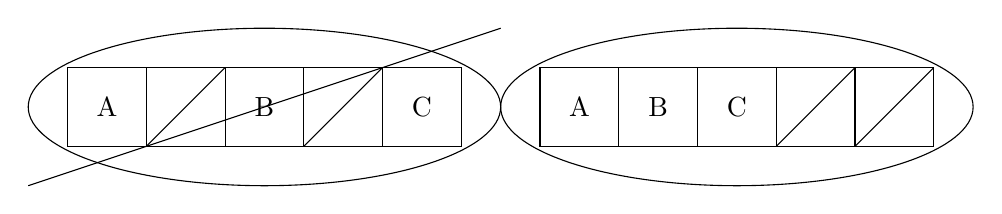
\begin{tikzpicture}[scale=2]
    \draw (.5,.5) rectangle  (3,1);
    \draw (1,.5) -- (1,1);
    \draw (1.5,.5) -- (1.5,1);
    \draw (2,.5) -- (2,1);
    \draw (2.5,.5) -- (2.5,1);
    \draw (1.75,.75) ellipse (1.5 and .5);
    \node at (.75,.75) {A};
    \draw (1,.5) -- (1.5,1);
    \node at (1.75,.75) {B};
    \draw (2,.5) -- (2.5,1);
    \node at (2.75,.75) {C};
    \draw (.25,.25) -- (3.25,1.25);

    \draw (3.5,.5) rectangle  (6,1);
    \draw (4,.5) -- (4,1);
    \draw (4.5,.5) -- (4.5,1);
    \draw (5,.5) -- (5,1);
    \draw (5.5,.5) -- (5.5,1);
    \draw (4.75,.75) ellipse (1.5 and .5);
    \node at (3.75,.75) {A};
    \draw (5,.5) -- (5.5,1);
    \node at (4.25,.75) {B};
    \draw (5.5,.5) -- (6,1);
    \node at (4.75,.75) {C};
  \end{tikzpicture}
  \caption{We force all None's to the end of the schedule, for simpler constraints.}
  \label{fig:none-constraints}
\end{figure}

Now that we have encoded
the notion of assignment of tasks to time steps
into constraints,
we must encode the timing constraints.
But how long does traveling between tasks task?
Due to the unpredictability of the robot and its environment,
we don't have a fixed bound on how long traveling between locations will take.
However, we do have a notion of the longest they should take
if nothing goes terribly wrong.
To simplify the scheduling,
we decided to ask the scheduler to only produce
schedules where DUB-E will always have enough travel time
if nothing goes terribly wrong.
If something \textit{does} go terribly wrong,
and DUB-E falls behind schedule,
we reschedule.
Here, we slightly compromise on optimality,
but we hope that the failure rate
will be low enough that
it won't be significantly worse in practice.
This is one of the realities of robotics, where
software and hardware must constantly be evaluating
and acting upon the environment, while also being mobile.
This makes almost all tasks unpredictable.

Once we have decided on an effective travel time,
we create two Int variables for each time step.
The first is the previously mentioned waitBefore,
the amount of time waited after finishing the last step
before starting the next one.
This variable is constrained to be non-negative,
but is otherwise free to be assigned whatever value
makes the schedule work out best.

The second Int variable
is the time at which that step is started.
This variable is constrained
to be exactly equal to the time
of the previous time variable,
plus the waitBefore time,
plus the time taken to complete the previous task,
plus the time taken to travel
from the previous task to the next task.
We encode the time taken to complete the previous task
using the ``ite'' construct for each possible previous task,
giving a zero value if that task was not completed last time step,
and the value of the task duration if it was.
We similarly encode the travel time,
using every possible pair of tasks we could have traveled in between.
Next, we require that if a task is done at a particular time step,
we require that that time step be fully within one of the tasks intervals.
That means that the task must start after the beginning of the interval,
and be finished before the end.

Finally, once we have properly constrained the solver
so that every solution will be a valid schedule,
that the robot can execute,
we attempt to find the \textit{optimal} schedule.
We decided to encode task weights as integers,
where higher is better,
but zero is an admin task.

First, we create a variable
for each task being accomplished
at some time step,
and set up an implication constraint
so that it can only be true
if the task was completed at some time step.
Then, we use a MaxSAT algorithm
to determine the schedule which can fit in the most admin tasks.
Then, we run it again to find the schedule with the greatest
sum weights of non-admin tasks,
given that it must accomplish the admin tasks found.
We reimplemented the WMax algorithm
as described in vZ, an extension to Z3 supporting MaxSAT \cite{vZ},
because we were not able to find the tool itself.
This approach is slightly flawed,
since there may be multiple optimal sets of admin tasks,
and one may allow more non-admin tasks,
but we felt that the slight benefits
of trying multiple configurations of optimal admin tasks
did not outweigh the running time cost.

Once we've figured out the optimal configuration,
we parse the list booleans
indicating whether each task was accomplished at each time step,
plus the waitBefore times of each step,
into a path, and give it to the ROS interface.


\section{Results}
A large portion of the unknowns and design
challenges in this project were related to
actually trying to get the new scheduler to
run in the current implementation of the SARA
system which is a series of python packages
built within the ROS environment. The first
challenge was to meet with the SARA project
leaders, Andrzej Pronobis and Michael Jae-Yoon
Chung. In a few early meetings, we expressed
interest in a delivery system for DUB-E and we
eventually settled on a generic task scheduling
problem as their current FIFO implementation was
supposed to be temporary.

Several meetings had to take place after choosing
a specific project while we developed designs.
This included two separate problems. One was to
come up with the details of the scheduling problem
itself and to settle on specifically what constraints
were important to the SARA team along with what was
interesting for us in our own goals. The other problem
involved determining how the scheduler would actually
be implemented in the current SARA code base. Several
problems were immediately raised. The most obvious was
the package design. ROS is built as a series of networks
calls and is built to be almost a pure event handling
system. This means we could not simply create a bunch
of classes and functions and dump them in. We had to come
up with service and message protocols and create independent
ROS nodes that could handle reading data from the network.
Figure~\ref{fig:ROSPackageDiag} gives a basic overview of
our resulting design. Another problem is that the SARA group
uses a Mongo database to communicate tasks information. This
was new to us so some additional outside knowledge was
required. One problem that became apparent later in the
project was the time consuming process of trying to create
tests for our code. Again, ROS makes this a bit difficult
as mock databases must be created, partial SARA code must be
launched, and test code gives very little feedback into problems
due to the ROS protocol. Finally, using the built in visualizer
was impossible in the current state of the SARA project
(explained later) and the visualizer we tried to use fought
us in more ways than one.

One of the main problems we faced
in the implementation of the encoding
was finding an appropriate MaxSAT algorithm.
We initially thought that there would be a simple
out-of-the-box solution with Z3.
But upon looking closer,
we found that the MaxSAT example
in the Z3 codebase
utilized special features of the C API,
and was not compatible with the current syntax.
Looking into the papers cited by the example,
it seemed like they only addressed the problem
for unweighted MaxSAT.
Instead, we researched and found the vZ paper,
and were able to implement some of the algorithms
it described,
although it took much longer than expected.

The final result was an encoder strong enough to
give more flexibility to the SARA project. The new
ROS package runs with 100\% integration with the SARA
code base in test cases. There are still a couple of
things that must be done before the new scheduler
can work live on the robot. As earlier discussed,
the old scheduler was extremely simple and did not take
into account any constraints except deadlines and these
were only looked at during runtime. Since we added much
complexity, there are a few integration issues to handle
before the robot can run live. Primarily, this means
providing a few more parameters in the database. We need
priorities and additional time constraints which we can
mock in testing and it can be simplified in live runs too.
For instance, we can just always assign priorities of 0
for now. The biggest hurdle is a useful ''World'' description.
Part of the encoder expects a World class which can give
back estimates of travel time and task time. This does
not exist yet, but the SARA team is currently working on
this, however it is a difficult problem, due to the
aforementioned chaos of real world robotics. The SARA
team is expecting to fully incorporate the new SAT encoder
into their project over the short time and we will
continue to support them.

Finally, we would like to document one result from the
project. Figure~\ref{fig:TenTaskResult} shows the outputted
plan of this encoder given ten tasks, chosen from three
possible distinguishable tasks for each location, and
ten locations, plus the start location. The red lines
demonstrate the resulting path beginning at ''startLoc''.
Table 1 shows the result in table format with tasks and wait
times.


\begin{figure}
\centering
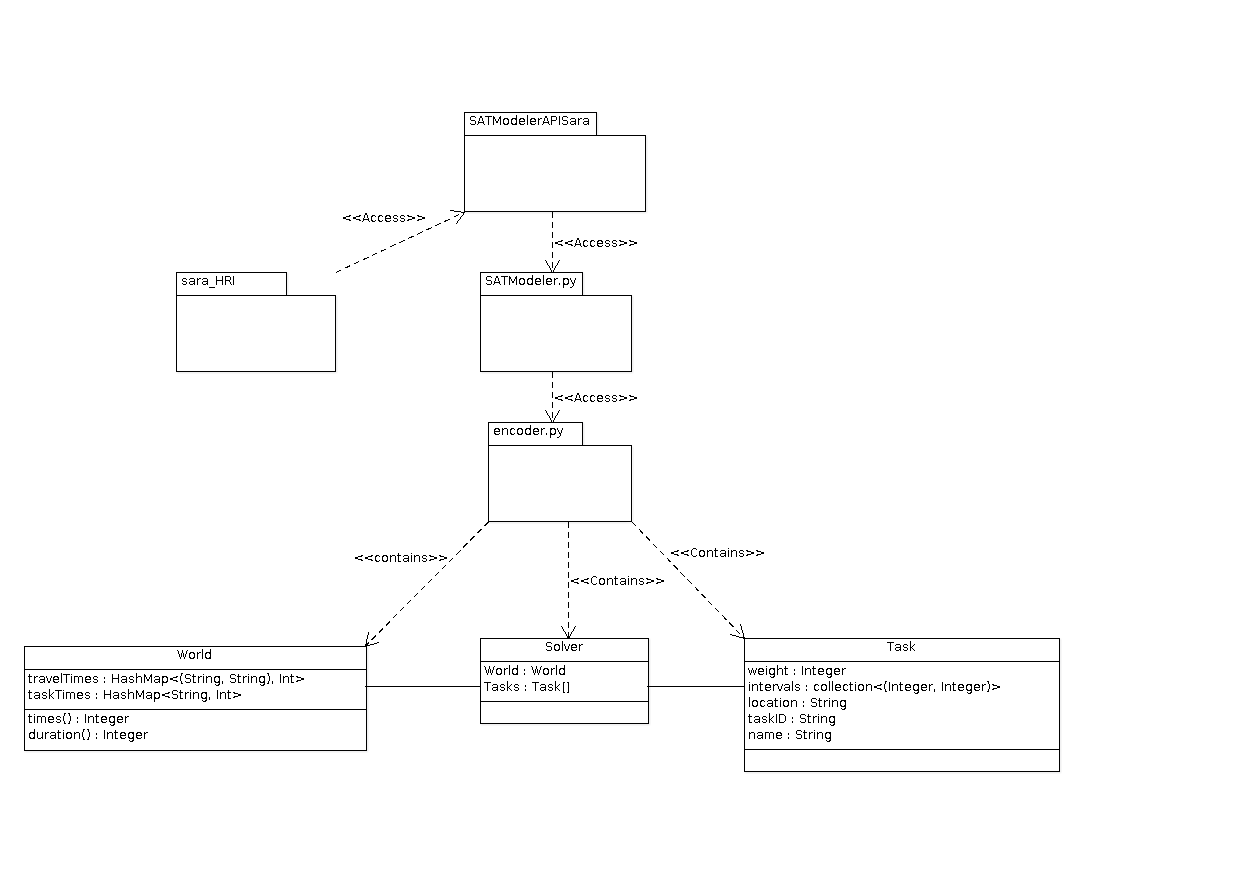
\includegraphics[width=0.8\textwidth]{ROS_Package_Diagram.png}
\caption{\label{fig:ROSPackageDiag}This is a package diagram of our ROS plugin for the SAT solver.}
\end{figure}

\begin{figure}
\centering
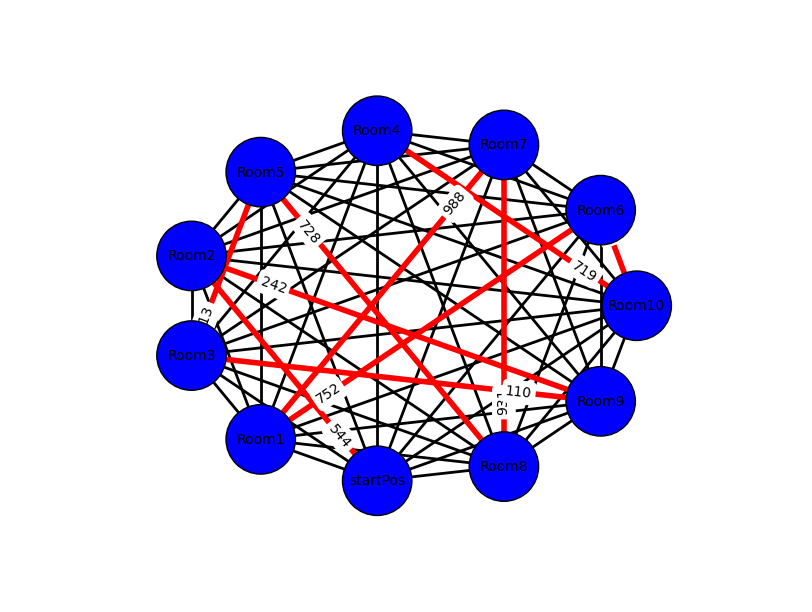
\includegraphics[width=0.8\textwidth]{Ten_Task_Result.png}
\caption{\label{fig:TenTaskResult}This is an example output of the sat scheduler given ten locations and ten jobs, one of three possible tasks at each location. Black lines are potential routes and red lines are the actual route. Numbers demonstrate time in seconds to travel that edge.}
\end{figure}

\begin{center}
    \begin{tabular}{ | p{7.5cm} | p{4.5cm} |}
    \hline
    Event & Time to Execute (seconds) \\ \hline \hline
    Wait at location ''startPos'' & 11034 \\ \hline
    Travel from location ''startPos'' to ''Room2'' & 544 \\ \hline
    Due Task3 at location ''Room2'' & 600 \\ \hline
    
    Wait at location ''Room2'' & 32564 \\ \hline
    Travel from location ''Room2'' to ''Room9'' & 242 \\ \hline
    Due Task1 at location ''Room9'' & 150 \\ \hline
    
    Wait at location ''Room9'' & 27021 \\ \hline
    Travel from location ''Room9'' to ''Room3'' & 110 \\ \hline
    Due Task1 at location ''Room3'' & 150 \\ \hline
    
    Wait at location ''Room3'' & 27457 \\ \hline
    Travel from location ''Room3'' to ''Room5'' & 713 \\ \hline
    Due Task2 at location ''Room5'' & 400 \\ \hline
    
    Wait at location ''Room5'' & 11951 \\ \hline
    Travel from location ''Room5'' to ''Room8'' & 728 \\ \hline
    Due Task3 at location ''Room8'' & 600 \\ \hline
    
    Wait at location ''Room8'' & 53709 \\ \hline
    Travel from location ''Room8'' to ''Room7'' & 931 \\ \hline
    Due Task2 at location ''Room7'' & 400 \\ \hline
    
    Wait at location ''Room7'' & 15881 \\ \hline
    Travel from location ''Room7'' to ''Room1'' & 988 \\ \hline
    Due Task2 at location ''Room1'' & 400 \\ \hline
    
    Wait at location ''Room1'' & 46943 \\ \hline
    Travel from location ''Room1'' to ''Room6'' & 752 \\ \hline
    Due Task1 at location ''Room6'' & 150 \\ \hline
    
    Wait at location ''Room6'' & 29825 \\ \hline
    Travel from location ''Room6'' to ''Room10'' & 416 \\ \hline
    Due Task3 at location ''Room10'' & 600 \\ \hline
    
    Wait at location ''Room10'' & 19836 \\ \hline
    Travel from location ''Room10'' to ''Room4'' & 719 \\ \hline
    Due Task2 at location ''Room4'' & 400 \\ \hline
    
    Done & 0 \\ \hline
    \end{tabular}
\end{center}

\section{Project Division}
For the most part we roughly divided the work into the encoding,
and the interface with DUB-E.
Skyler handled the interface with the robot,
setting up ROS nodes and working with Michael and Andrzej
to get the encoder integrated
into the DUB-E codebase. This required significant
domain knowledge and experience working with the
''Robotic Operating System'' or ROS in which the
current SARA code base is implemented in.
Alex handled the actual encoding of the task constraints,
setting up the Z3 bindings to interface with the code,
and writing modules to take in task information,
encode it into a set of Z3 constraints,
decode the Z3 output into a schedule,
and format the schedule for DUB-E.


\section{Applied Topics}
This project involved mostly topics
that we discussed at the beginning of the quarter,
although it of course was supported by
the work we did throughout the quarter.
Specifically, the work on encoding different types of constraints
into conjunctive normal form was paramount to the project.
The encoding also made heavy use of MaxSAT,
which we touched on in class,
to satisfy the greatest number of tasks
in cases where not all tasks could be satisfied.


\begin{thebibliography}{9}

\bibitem{vZ}
  Bj{\o}rner, Nikolaj and Phan, Anh-Dung,
  \emph{vZ: Maximal Satisfaction with Z3}.
  http://research.microsoft.com/en-US/people/nbjorner/scss2014.pdf
  2014.

\bibitem{z3}
  De Moura, Leonardo and Bj{\o}rner, Nikolaj,
  \emph{Z3: An Efficient SMT Solver}.
  Springer-Verlag,
  2008.

\bibitem{MongoDB}
  \emph{MongoDB}.
  http://www.mongodb.org/

\bibitem{ROS}
  \emph{ROS: Robotic Operating System}.
  http://wiki.ros.org/

\bibitem{SARA}
  \emph{SARA: Semantics Aware Robotic Assistant}.

\end{thebibliography}
\end{document}
